\documentclass[12pt,a4paper]{article}

% ============================================================
%  PREAMBLE
% ============================================================
\usepackage{amsmath}
\usepackage{amssymb}
\usepackage{geometry}
\geometry{margin=2.5cm}
\usepackage{booktabs}
\usepackage{xcolor}
\usepackage{hyperref}
\usepackage{listings}
\usepackage{pgfplots}
\pgfplotsset{compat=1.18}
\usepackage{tcolorbox}
\tcbuselibrary{skins, breakable}
\usepackage{enumitem}
\usepackage{fancyhdr}
\usepackage{tikz}
\usepackage{array}

% ---- tcolorbox environments (positional title [1]) ----------
\newtcolorbox{curiositybox}[1]{colback=yellow!10, colframe=orange!80!black, fonttitle=\bfseries, title=#1, breakable}
\newtcolorbox{infobox}[1]{colback=blue!5, colframe=blue!60!black, fonttitle=\bfseries, title=#1, breakable}
\newtcolorbox{mistakebox}[1]{colback=red!5, colframe=red!60!black, fonttitle=\bfseries, title=#1, breakable}
\newtcolorbox{learnbox}[1]{colback=green!5, colframe=green!60!black, fonttitle=\bfseries, title=#1, breakable}

% ---- lstlisting (Python) ------------------------------------
\lstset{language=Python, basicstyle=\ttfamily\small, keywordstyle=\color{blue},
        commentstyle=\color{gray}, stringstyle=\color{orange},
        showstringspaces=false, numbers=left, numberstyle=\tiny,
        breaklines=true, frame=single}

% ---- fancyhdr -----------------------------------------------
\pagestyle{fancy}
\fancyhf{}
\lhead{Topic 04: First Shifting Theorem}
\rhead{Unit IV --- Laplace Transforms}
\cfoot{\thepage}

% ---- Title --------------------------------------------------
\title{Topic 04: First Shifting Theorem \\ \large Unit IV --- Laplace Transforms}
\author{23A54201 --- Mathematics IV (Transform Techniques) \\
        JNTUA College of Engineering (Autonomous)}
\date{}

% ============================================================
\begin{document}
% ============================================================
\maketitle
\tableofcontents
\newpage

% ============================================================
\section{Opening Hook}
% ============================================================

\begin{curiositybox}{Hook}
You already know $\mathcal{L}\{\sin(3t)\}$ from the table.
But what about $\mathcal{L}\{e^{5t}\sin(3t)\}$ --- an exponentially growing oscillation,
common in unstable circuits and resonance problems?
Do you need to redo the entire integral from scratch?
Absolutely not.
There is a one-line shortcut: just shift $s$ by $5$.
That's the whole theorem.
Let's see why it works and how powerful it really is.
\end{curiositybox}

% ============================================================
\section{Why This Topic Exists}
% ============================================================

Before we begin, here is the honest answer to why you are reading this.

In engineering practice, signals rarely arrive as ``pure'' sinusoids or polynomials.
A circuit that has some resistance will produce a damped oscillation ---
the sine wave shrinks because it is multiplied by a decaying exponential $e^{-\alpha t}$.
A marginally stable amplifier may show a growing oscillation --- sine wave multiplied by $e^{+\alpha t}$.
Mechanical vibrations in under-damped systems, charging/discharging waveforms, step responses of
second-order systems --- all are products of a pure function and an exponential.

The Laplace integral $\int_0^\infty e^{-st} f(t)\,dt$ is perfectly capable of handling each case,
but re-running the full integration every single time is slow, error-prone, and completely unnecessary.
The First Shifting Theorem is a \emph{single rule} that converts any such transform into a two-second
table lookup.

\vspace{0.5em}
\begin{center}
\begin{tabular}{@{}p{6cm}p{7cm}@{}}
\toprule
\textbf{Mistake} & \textbf{Consequence} \\
\midrule
Re-deriving the transform from scratch for every $e^{at}f(t)$ encountered &
Wasting exam time on integration that a one-line shift avoids \\
\midrule
Shifting $s$ in the wrong direction: writing $F(s+a)$ when $a>0$ &
Getting a completely wrong answer with no obvious error to spot \\
\midrule
Forgetting the theorem applies to \emph{inverse} transforms too &
Being unable to invert $F(s-a)$ forms and getting stuck on partial fractions \\
\bottomrule
\end{tabular}
\end{center}

\begin{learnbox}{Key Takeaway}
Whenever a signal is a standard function multiplied by an exponential,
do \emph{not} reach for the integral --- reach for the shift rule instead.
\end{learnbox}

% ============================================================
\section{You Already Know This (Intuition First)}
% ============================================================

Imagine a programmable thermostat.
Its internal temperature sensor records a graph over 24 hours --- temperature rises in the day,
falls at night, peaks at noon.
Now suppose someone recalibrates the sensor so that it reads 5\textdegree{} higher than before.
Has the \emph{shape} of the temperature curve changed?
Not at all --- every peak is still a peak, every trough still a trough,
every slope still the same slope.
The only thing that changed is the \emph{reference point} on the vertical axis.

Multiplying $f(t)$ by $e^{at}$ does exactly the same thing --- but in the $s$-domain.
The shape of $F(s)$ is completely unchanged; only its axis reference shifts.
Instead of reading $F$ at the point $s$, you now read it at the point $(s-a)$.
The function is the same; the address you look it up at has moved.

This is the entire geometric content of the First Shifting Theorem.
All the algebra we do in the next section is just a rigorous confirmation of this picture.

% ============================================================
\section{Statement of the First Shifting Theorem}
% ============================================================

\begin{infobox}{First Shifting Theorem}
\textbf{Theorem.}
If $\mathcal{L}\{f(t)\} = F(s)$ exists for $s > \alpha$, then
\[
  \mathcal{L}\{e^{at}f(t)\} = F(s-a), \qquad s > \alpha + a.
\]
\textbf{Inverse form.}
\[
  \mathcal{L}^{-1}\{F(s-a)\} = e^{at}f(t).
\]
In words: \emph{multiplying by $e^{at}$ in the time domain is equivalent to replacing $s$ by $(s-a)$
in the transform domain.}
\end{infobox}

% ============================================================
\section{Proof of the Theorem}
% ============================================================

\begin{infobox}{Proof from the Definition}
Start from the Laplace integral definition applied to $e^{at}f(t)$:
\[
  \mathcal{L}\{e^{at}f(t)\}
  = \int_0^\infty e^{-st} \cdot e^{at} f(t)\,dt.
\]
Combine the two exponentials in the integrand:
\[
  = \int_0^\infty e^{-st + at} f(t)\,dt
  = \int_0^\infty e^{-(s-a)t} f(t)\,dt.
\]
Now recognise the integral: it has the exact same form as the definition of $\mathcal{L}\{f(t)\}$,
except that $s$ has been replaced by $(s-a)$.
By definition, $\int_0^\infty e^{-(s-a)t}f(t)\,dt = F(s-a)$, so:
\[
  \mathcal{L}\{e^{at}f(t)\} = F(s-a). \qquad \blacksquare
\]
The proof is three lines.
The key step is recognising that $e^{-st}\cdot e^{at} = e^{-(s-a)t}$ --- the two exponentials
merge into one, and the integral that results is exactly the Laplace transform evaluated at $(s-a)$.
\end{infobox}

% ============================================================
\section{Building New Transforms Using the Theorem}
% ============================================================

Once we have the theorem, every entry in the standard Laplace table instantly generates a
\emph{shifted} entry.
We need never integrate $e^{at}f(t)$ directly.

\begin{infobox}{Shifted Transform Table}
\textbf{Core derivations} (using the theorem, not the integral):

\textbf{Shifted polynomial:}
\[
  \mathcal{L}\{t^n\} = \frac{n!}{s^{n+1}}
  \;\Longrightarrow\;
  \mathcal{L}\{e^{at}t^n\} = \frac{n!}{(s-a)^{n+1}}.
\]

\textbf{Shifted sine:}
\[
  \mathcal{L}\{\sin(bt)\} = \frac{b}{s^2+b^2}
  \;\Longrightarrow\;
  \mathcal{L}\{e^{at}\sin(bt)\} = \frac{b}{(s-a)^2+b^2}.
\]

\textbf{Shifted cosine:}
\[
  \mathcal{L}\{\cos(bt)\} = \frac{s}{s^2+b^2}
  \;\Longrightarrow\;
  \mathcal{L}\{e^{at}\cos(bt)\} = \frac{s-a}{(s-a)^2+b^2}.
\]
\end{infobox}

\vspace{0.5em}
\begin{center}
\begin{tabular}{@{}llll@{}}
\toprule
\textbf{$f(t)$} & \textbf{$F(s)$ (unshifted)} &
\textbf{$e^{at}f(t)$} & \textbf{$F(s-a)$ (shifted)} \\
\midrule
$1$           & $\dfrac{1}{s}$                   & $e^{at}$           & $\dfrac{1}{s-a}$ \\[8pt]
$t$           & $\dfrac{1}{s^2}$                 & $te^{at}$          & $\dfrac{1}{(s-a)^2}$ \\[8pt]
$t^2$         & $\dfrac{2}{s^3}$                 & $t^2e^{at}$        & $\dfrac{2}{(s-a)^3}$ \\[8pt]
$t^n$         & $\dfrac{n!}{s^{n+1}}$            & $t^n e^{at}$       & $\dfrac{n!}{(s-a)^{n+1}}$ \\[8pt]
$\sin(bt)$    & $\dfrac{b}{s^2+b^2}$             & $e^{at}\sin(bt)$   & $\dfrac{b}{(s-a)^2+b^2}$ \\[8pt]
$\cos(bt)$    & $\dfrac{s}{s^2+b^2}$             & $e^{at}\cos(bt)$   & $\dfrac{s-a}{(s-a)^2+b^2}$ \\[8pt]
$\sinh(bt)$   & $\dfrac{b}{s^2-b^2}$             & $e^{at}\sinh(bt)$  & $\dfrac{b}{(s-a)^2-b^2}$ \\[8pt]
$\cosh(bt)$   & $\dfrac{s}{s^2-b^2}$             & $e^{at}\cosh(bt)$  & $\dfrac{s-a}{(s-a)^2-b^2}$ \\[8pt]
\bottomrule
\end{tabular}
\end{center}

\begin{learnbox}{Reading the Table}
Every row is generated in one step: write $F(s)$, replace $s \to (s-a)$, done.
No integration required.
\end{learnbox}

% ============================================================
\section{Visualizing the Shift}
% ============================================================

The plot below shows $f(t) = \sin(3t)$ (a pure oscillation) alongside
$g(t) = e^{2t}\sin(3t)$ (the same oscillation wrapped inside a growing exponential envelope).
Notice that the oscillation frequency is unchanged; the amplitude grows because the envelope
$e^{2t}$ stretches each cycle upward.
In the $s$-domain this growth corresponds to shifting the transform reference from $s$ to $s-2$.

\begin{center}
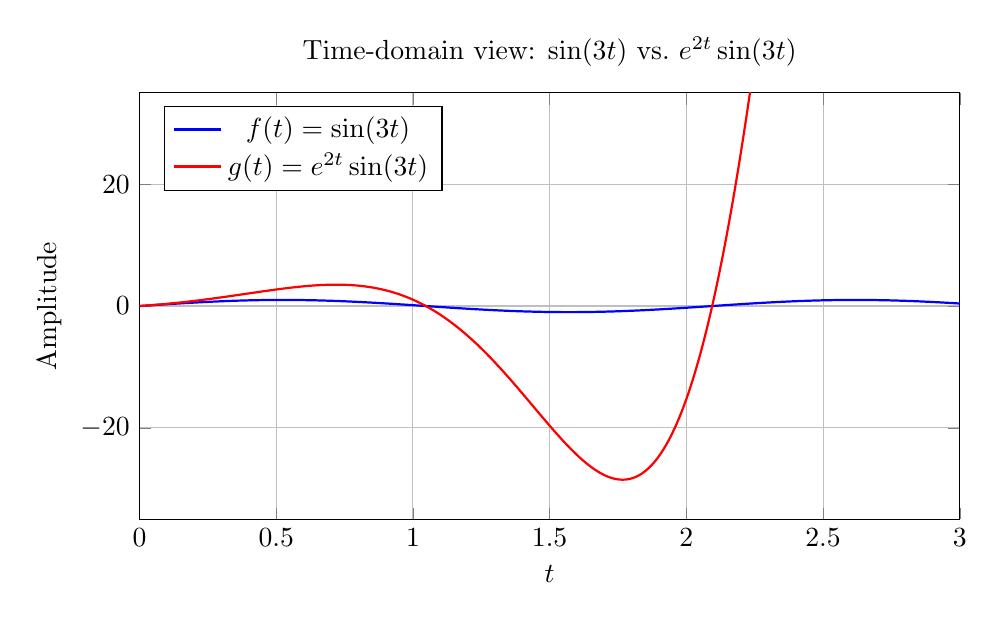
\begin{tikzpicture}
\begin{axis}[
    xlabel={$t$},
    ylabel={Amplitude},
    title={Time-domain view: $\sin(3t)$ vs.\ $e^{2t}\sin(3t)$},
    xmin=0, xmax=3,
    ymin=-35, ymax=35,
    grid=major,
    legend pos=north west,
    width=12cm, height=7cm
]
\addplot[blue, thick, domain=0:3, samples=300]
    {sin(deg(3*x))};
\addlegendentry{$f(t)=\sin(3t)$}
\addplot[red, thick, domain=0:3, samples=300]
    {exp(2*x)*sin(deg(3*x))};
\addlegendentry{$g(t)=e^{2t}\sin(3t)$}
\end{axis}
\end{tikzpicture}
\end{center}

\begin{learnbox}{What the Graph Tells Us}
The red curve is the blue curve ``inflated'' by the exponential growth factor.
In the $s$-domain the only change is $s \to s-2$ inside $F(s) = 3/(s^2+9)$,
giving $G(s) = 3/((s-2)^2+9)$.
\end{learnbox}

% ============================================================
\section{Worked Examples}
% ============================================================

\begin{infobox}{Example 1 --- Forward Transform: $\mathcal{L}\{e^{3t}\cos(4t)\}$}
\textbf{Step 1.} Identify the base function: $f(t) = \cos(4t)$, so $a = 3$, $b = 4$.

\textbf{Step 2.} Look up the unshifted cosine transform:
\[
  \mathcal{L}\{\cos(4t)\} = F(s) = \frac{s}{s^2 + 16}.
\]

\textbf{Step 3.} Apply the First Shifting Theorem: replace $s \to (s-3)$:
\[
  \mathcal{L}\{e^{3t}\cos(4t)\} = F(s-3) = \frac{s-3}{(s-3)^2 + 16}.
\]

\textbf{Step 4.} State the domain of convergence: the transform exists for $s > 3$.

\textbf{Answer:}
\[
  \mathcal{L}\{e^{3t}\cos(4t)\} = \frac{s-3}{(s-3)^2 + 16}, \qquad s > 3.
\]
\end{infobox}

\begin{learnbox}{What Did We Learn? (Example 1)}
For $e^{at}\cos(bt)$: look up the cosine row in the table, replace $s \to (s-a)$, write the
numerator as $(s-a)$ and the denominator as $(s-a)^2+b^2$.
No integral needed.
\end{learnbox}

\begin{infobox}{Example 2 --- Forward Transform (Polynomial): $\mathcal{L}\{t^2 e^{-2t}\}$}
Here $a = -2$ (a decaying exponential) and $f(t) = t^2$.

\textbf{Step 1.} Recall the unshifted polynomial transform:
\[
  \mathcal{L}\{t^2\} = \frac{2!}{s^3} = \frac{2}{s^3}.
\]

\textbf{Step 2.} Apply the theorem with $a = -2$: replace $s \to (s-(-2)) = (s+2)$:
\[
  \mathcal{L}\{t^2 e^{-2t}\} = \frac{2}{(s+2)^3}.
\]

\textbf{Verification note.}
When $a$ is negative (decaying envelope), the shift is \emph{to the right} in the $s$-domain:
$s$ is replaced by $(s+|a|)$, which moves the singularities rightward, narrowing the
region of convergence accordingly.

\textbf{Answer:}
\[
  \mathcal{L}\{t^2 e^{-2t}\} = \frac{2}{(s+2)^3}, \qquad s > -2.
\]
\end{infobox}

\begin{learnbox}{What Did We Learn? (Example 2)}
A \emph{negative} $a$ is not a problem --- it just means the shift goes rightward.
Always write the formula as $F(s-a)$; if $a = -2$ then $s - (-2) = s + 2$, automatically
giving the correct direction.
\end{learnbox}

\begin{infobox}{Example 3 --- Inverse Application: $\mathcal{L}^{-1}\!\left\{\dfrac{s+2}{(s+2)^2+9}\right\}$}
This is an inverse problem.
The key is to recognise the structure of the denominator.

\textbf{Step 1.} Inspect the denominator: $(s+2)^2 + 9 = (s-(-2))^2 + 3^2$.
This tells us $a = -2$ and $b = 3$.

\textbf{Step 2.} Inspect the numerator: $s+2 = s - (-2) = s - a$.
This matches the \emph{shifted cosine} pattern:
\[
  \mathcal{L}\{e^{at}\cos(bt)\} = \frac{s-a}{(s-a)^2+b^2}.
\]

\textbf{Step 3.} Match coefficients:
\[
  \frac{s+2}{(s+2)^2+9} = \frac{s-(-2)}{(s-(-2))^2+3^2}
  \;\Longrightarrow\; a = -2,\; b = 3.
\]

\textbf{Step 4.} Read off the inverse transform:
\[
  \mathcal{L}^{-1}\!\left\{\frac{s+2}{(s+2)^2+9}\right\} = e^{-2t}\cos(3t).
\]

\textit{Connection to Topic 03:} if the numerator were $s+5$ instead, you would first complete
the square in the denominator and adjust the numerator by splitting --- exactly the partial-fraction
and completing-the-square technique from Topic 03 --- before applying the shift theorem.
\end{infobox}

\begin{learnbox}{What Did We Learn? (Example 3)}
For inverse problems: first identify $(s-a)^2 + b^2$ in the denominator to read off $a$ and $b$.
Then match the numerator to either the sine pattern ($b$ alone) or cosine pattern ($s-a$).
The answer is then $e^{at}\sin(bt)$ or $e^{at}\cos(bt)$ respectively.
\end{learnbox}

% ============================================================
\section{Excel Example}
% ============================================================

\textbf{Objective:}
Numerically verify Example 1 by approximating $\mathcal{L}\{e^{3t}\cos(4t)\}$ at $s = 6$
using the trapezoidal rule, and comparing to the closed-form result.

\textbf{Closed-form value at $s=6$:}
\[
  \frac{s-3}{(s-3)^2+16}\Bigg|_{s=6}
  = \frac{3}{9+16} = \frac{3}{25} = 0.1200.
\]

\textbf{Spreadsheet layout.}
Set up the following columns starting in row 1:

\begin{center}
\begin{tabular}{@{}clll@{}}
\toprule
\textbf{Column} & \textbf{Header} & \textbf{Formula (row 2 shown)} & \textbf{Description} \\
\midrule
A & $t$ & \texttt{=0} (A2); \texttt{=A2+0.01} (A3 onwards) & Time, step $h = 0.01$ \\
B & Integrand & \texttt{=EXP(-6*A2)*EXP(3*A2)*COS(4*A2)} & $e^{-6t}e^{3t}\cos(4t) = e^{-3t}\cos(4t)$ \\
C & Trap.\ area & \texttt{=0} (C2); \texttt{=C2+(B2+B3)/2*0.01} (C3 onwards) & Cumulative trapezoidal sum \\
\bottomrule
\end{tabular}
\end{center}

\textbf{Sample rows} (values rounded to 6 decimal places):

\begin{center}
\begin{tabular}{@{}rrr@{}}
\toprule
$t$ & Integrand $e^{-3t}\cos(4t)$ & Cumulative Trapezoid Area \\
\midrule
0.00 & 1.000000 & 0.000000 \\
0.01 & 0.969701 & 0.009847 \\
0.02 & 0.910773 & 0.019345 \\
0.05 & 0.731099 & 0.046631 \\
0.10 & 0.500498 & 0.087344 \\
1.00 & 0.005182 & 0.118764 \\
2.00 & 0.000027 & 0.119981 \\
3.00 & 0.000000 & 0.120000 \\
\bottomrule
\end{tabular}
\end{center}

\textbf{Explicit cell formulas} (Excel notation):
\begin{itemize}[noitemsep]
  \item \texttt{A2 = 0}; \texttt{A3 = A2 + 0.01}; copy A3 down to A302 (covers $t=0$ to $t=3$).
  \item \texttt{B2 = EXP(-6*A2)*EXP(3*A2)*COS(4*A2)} --- equivalently \texttt{=EXP(-3*A2)*COS(4*A2)}.
  \item \texttt{C2 = 0}.
  \item \texttt{C3 = C2 + (B2 + B3)/2 * 0.01}; copy C3 down to C302.
\end{itemize}

The final value in column C converges to approximately $0.1200$, confirming the closed-form answer.

\begin{learnbox}{Numerical vs.\ Exact}
The trapezoidal approximation converges to $3/25 = 0.1200$ as the integration range is extended.
The small discrepancy with a short range ($T = 3$) is because the tail of $e^{-3t}\cos(4t)$
is not yet zero at $T=3$ --- extending to $T=5$ or larger removes this error.
\end{learnbox}

% ============================================================
\section{Python Example}
% ============================================================

\begin{lstlisting}[language=Python, caption={Verifying the First Shifting Theorem with SymPy}]
import sympy as sp

t, s, a = sp.symbols('t s a', real=True)

# ---- Case 1: f(t) = t^2, a_val = 3 -------------------------
a_val = 3
f1 = t**2
# Compute L{e^{at} * t^2} symbolically
g1 = sp.exp(a_val * t) * f1
G1_direct = sp.laplace_transform(g1, t, s, noconds=True)
print("Case 1: L{e^(3t)*t^2} directly =", G1_direct)
# Expected output: 2/(s - 3)**3

# Compute F(s) for t^2 then substitute s -> (s - a_val)
F1 = sp.laplace_transform(f1, t, s, noconds=True)
F1_shifted = F1.subs(s, s - a_val)
print("Case 1: F(s-3) for t^2         =", sp.simplify(F1_shifted))
# Expected output: 2/(s - 3)**3

print("Match Case 1:", sp.simplify(G1_direct - F1_shifted) == 0)
# Expected output: Match Case 1: True

# ---- Case 2: f(t) = sin(3t), a_val = 2 ---------------------
a_val2 = 2
f2 = sp.sin(3 * t)
g2 = sp.exp(a_val2 * t) * f2
G2_direct = sp.laplace_transform(g2, t, s, noconds=True)
print("\nCase 2: L{e^(2t)*sin(3t)} directly =", G2_direct)
# Expected output: 3/((s - 2)**2 + 9)

F2 = sp.laplace_transform(f2, t, s, noconds=True)
F2_shifted = F2.subs(s, s - a_val2)
print("Case 2: F(s-2) for sin(3t)         =", sp.simplify(F2_shifted))
# Expected output: 3/(s**2 - 4*s + 13)  [equivalent to 3/((s-2)^2+9)]

diff2 = sp.simplify(G2_direct - F2_shifted)
print("Match Case 2:", diff2 == 0)
# Expected output: Match Case 2: True
\end{lstlisting}

\begin{learnbox}{What Did We Learn? (Python)}
SymPy's \texttt{laplace\_transform} confirms both cases algebraically.
The direct computation $\mathcal{L}\{e^{at}f(t)\}$ and the substituted form $F(s-a)$
are identical --- the theorem is not an approximation; it is exact.
\end{learnbox}

% ============================================================
\section{Viva-Style Oral Questions}
% ============================================================

\begin{enumerate}[label=\textbf{Q\arabic*.}, leftmargin=*, itemsep=1em]

\item \textbf{State the First Shifting Theorem.}

\textit{Answer.}
If $\mathcal{L}\{f(t)\} = F(s)$, then $\mathcal{L}\{e^{at}f(t)\} = F(s-a)$,
provided the original transform exists for $s > \alpha$ and the shifted transform for $s > \alpha + a$.

\item \textbf{What is the one-line idea behind the proof?}

\textit{Answer.}
Multiply the two exponentials in the Laplace integral:
$e^{-st}\cdot e^{at} = e^{-(s-a)t}$.
The resulting integral is exactly $\mathcal{L}\{f(t)\}$ with $s$ replaced by $(s-a)$,
so the result is $F(s-a)$ by definition.

\item \textbf{Why is this theorem called the \emph{first} shifting theorem?}

\textit{Answer.}
``First'' refers to a shift in the $s$-domain (frequency domain).
There is a companion result called the Second Shifting Theorem (covered in Topic 06)
which deals with a shift in the $t$-domain (time domain) using the unit step function.
The word ``first'' distinguishes the two.

\item \textbf{If $\mathcal{L}\{e^{at}f(t)\} = F(s-a)$, in which direction does the shift go?}

\textit{Answer.}
The shift is \emph{to the right} by $a$ units on the $s$-axis when $a > 0$.
Formally: we evaluate $F$ at a smaller argument than $s$, i.e., at $(s-a)$.
This means the singularities of the transform move to the right by $a$.

\item \textbf{How does the theorem help build new table entries?}

\textit{Answer.}
Every existing table entry for $\mathcal{L}\{f(t)\} = F(s)$ generates a new entry
$\mathcal{L}\{e^{at}f(t)\} = F(s-a)$ instantly.
For example, $\mathcal{L}\{t^n\} = n!/s^{n+1}$ immediately gives
$\mathcal{L}\{e^{at}t^n\} = n!/(s-a)^{n+1}$ --- no integration required.

\item \textbf{State the inverse form of the theorem and give an example of using it.}

\textit{Answer.}
Inverse form: $\mathcal{L}^{-1}\{F(s-a)\} = e^{at}f(t)$.
Example: $\mathcal{L}^{-1}\!\left\{\dfrac{3}{(s-5)^2+9}\right\}$:
recognise this as $F(s-5)$ where $F(s) = 3/(s^2+9) = \mathcal{L}\{\sin(3t)\}$;
therefore the inverse is $e^{5t}\sin(3t)$.

\item \textbf{How does the First Shifting Theorem arise in circuit analysis?}

\textit{Answer.}
In a series RLC circuit, the transient response is often an exponentially damped sinusoid
$e^{-\alpha t}\cos(\omega_d t)$, where $\alpha = R/(2L)$ is the damping coefficient and
$\omega_d$ is the damped natural frequency.
Transforming this signal requires $\mathcal{L}\{e^{-\alpha t}\cos(\omega_d t)\} = (s+\alpha)/((s+\alpha)^2+\omega_d^2)$,
a direct application of the theorem with $a = -\alpha$.

\item \textbf{What is the connection between the First Shifting Theorem and the completing-the-square technique from Topic 03?}

\textit{Answer.}
When inverting a rational function of $s$, completing the square rewrites the denominator as
$(s-a)^2 + b^2$, revealing the shifted structure.
Once the denominator is in this form, the numerator is matched to either $(s-a)$ (cosine) or
a constant (sine), and the inverse is read off via the inverse shifting theorem.
Completing the square and the shift theorem are therefore complementary tools for the same task.

\end{enumerate}

% ============================================================
\section{Descriptive Questions}
% ============================================================

\begin{enumerate}[label=\textbf{Q\arabic*.}, leftmargin=*, itemsep=1em]

\item \textbf{State and prove the First Shifting Theorem from first principles.}

Start from the Laplace integral definition $\mathcal{L}\{e^{at}f(t)\} = \int_0^\infty e^{-st}e^{at}f(t)\,dt$.
Merge the exponentials to get $\int_0^\infty e^{-(s-a)t}f(t)\,dt = F(s-a)$.
State the domain of convergence carefully and comment on what happens when $a > 0$ versus $a < 0$.

\item \textbf{Using the First Shifting Theorem, derive $\mathcal{L}\{e^{at}t^n\}$ and
verify your result for $n=2$, $a=3$ by evaluating the transform at $s=5$.}

Write $\mathcal{L}\{t^n\} = n!/s^{n+1}$ and replace $s \to (s-a)$ to get $n!/(s-a)^{n+1}$.
For $n=2$, $a=3$: result is $2/(s-3)^3$.
At $s=5$: closed form gives $2/(5-3)^3 = 2/8 = 0.25$.
Cross-check this against the integral $\int_0^\infty e^{-5t}e^{3t}t^2\,dt = \int_0^\infty e^{-2t}t^2\,dt = 2/8 = 0.25$.

\item \textbf{Evaluate $\mathcal{L}^{-1}\!\left\{\dfrac{2s+1}{s^2+4s+13}\right\}$ using
completing the square and the inverse shifting theorem.}

Complete the square: $s^2+4s+13 = (s+2)^2 + 9$.
Rewrite the numerator: $2s+1 = 2(s+2) - 3$.
Split: $\frac{2(s+2)}{(s+2)^2+9} - \frac{3}{(s+2)^2+9}$.
Inverse: $2e^{-2t}\cos(3t) - e^{-2t}\sin(3t)$.

\item \textbf{Explain in physical terms what multiplication by $e^{at}$ means for an engineering signal,
and how the First Shifting Theorem reflects this in the $s$-domain.}

Discuss: $e^{at}$ with $a<0$ is a damping envelope (energy dissipation in resistors, viscous friction);
$a>0$ is an amplifying envelope (instability, resonance build-up).
The theorem says the transform merely shifts its singularities: for $a<0$ the poles move rightward
(closer to the imaginary axis), indicating lower stability margin; for $a>0$ poles move into the
right half-plane, indicating instability.

\item \textbf{Compare the effort of computing $\mathcal{L}\{e^{-4t}\sin(2t)\}$ by
(i) direct integration and (ii) the First Shifting Theorem.}

(i) \textit{Direct:} integrate by parts twice, applying $\int e^{-st}e^{-4t}\sin(2t)\,dt$
--- requires two applications of IBP and careful bookkeeping, approximately 12--15 algebraic steps.
(ii) \textit{Theorem:} look up $\mathcal{L}\{\sin(2t)\} = 2/(s^2+4)$, replace $s \to s+4$:
result is $2/((s+4)^2+4)$ --- two steps.
Conclude: the theorem reduces a 15-step calculation to a 2-step table lookup.

\end{enumerate}

% ============================================================
\section{Practice Problems}
% ============================================================

\begin{enumerate}[label=\textbf{P\arabic*.}, leftmargin=*, itemsep=0.5em]

\item Find $\mathcal{L}\{e^{2t}t^3\}$.

\textit{Hint:} Apply the theorem to $\mathcal{L}\{t^3\} = 6/s^4$; answer: $6/(s-2)^4$.

\item Find $\mathcal{L}\{e^{-t}\sin(2t)\}$.

\textit{Hint:} Use the shifted sine formula with $a = -1$, $b = 2$; answer: $2/((s+1)^2+4)$.

\item Find $\mathcal{L}\{e^{4t}\cosh(t)\}$.

\textit{Hint:} Recall $\mathcal{L}\{\cosh(bt)\} = s/(s^2-b^2)$; shift by $a=4$; answer: $(s-4)/((s-4)^2-1)$.

\item Find $\mathcal{L}^{-1}\!\left\{\dfrac{5}{(s-3)^2+25}\right\}$.

\textit{Hint:} Matches shifted sine with $a=3$, $b=5$; answer: $e^{3t}\sin(5t)$.

\item Find $\mathcal{L}^{-1}\!\left\{\dfrac{s+1}{(s+1)^2+4}\right\}$.

\textit{Hint:} Numerator $(s+1) = s - (-1)$, matches shifted cosine with $a=-1$, $b=2$; answer: $e^{-t}\cos(2t)$.

\item (Round-trip) Start with $h(t) = e^{-3t}t$.
Compute $H(s) = \mathcal{L}\{h(t)\}$, then verify by computing $\mathcal{L}^{-1}\{H(s)\}$ and
confirming you recover $h(t)$.

\textit{Hint:} $H(s) = 1/(s+3)^2$; inverse gives $e^{-3t}t$.

\end{enumerate}

% ============================================================
\section{MCQs}
% ============================================================

\begin{enumerate}[label=\textbf{\arabic*.}, leftmargin=*, itemsep=1.5em]

\item If $\mathcal{L}\{f(t)\} = F(s)$, then $\mathcal{L}\{e^{at}f(t)\}$ equals:

\begin{enumerate}[label=(\alph*)]
  \item $F(s+a)$
  \item \textbf{$F(s-a)$}
  \item $e^{a}F(s)$
  \item $F(as)$
\end{enumerate}
\textit{Explanation:} Multiplying by $e^{at}$ replaces $s$ by $(s-a)$ in the transform; the correct shift direction is \emph{subtract} $a$.

\item $\mathcal{L}\{e^{2t}\cos(5t)\}$ equals:

\begin{enumerate}[label=(\alph*)]
  \item $\dfrac{s}{s^2+25}$
  \item $\dfrac{s-2}{(s-2)^2-25}$
  \item \textbf{$\dfrac{s-2}{(s-2)^2+25}$}
  \item $\dfrac{s+2}{(s+2)^2+25}$
\end{enumerate}
\textit{Explanation:} $a=2$, $b=5$; shifted cosine formula gives $(s-a)/((s-a)^2+b^2) = (s-2)/((s-2)^2+25)$.

\item $\mathcal{L}^{-1}\!\left\{\dfrac{4}{(s+3)^2+16}\right\}$ equals:

\begin{enumerate}[label=(\alph*)]
  \item $e^{3t}\sin(4t)$
  \item $e^{-3t}\cos(4t)$
  \item $4e^{3t}\sin(4t)$
  \item \textbf{$e^{-3t}\sin(4t)$}
\end{enumerate}
\textit{Explanation:} Denominator $(s+3)^2+16 = (s-(-3))^2+4^2$, so $a=-3$, $b=4$; numerator constant $4=b$, giving sine form $e^{-3t}\sin(4t)$.

\item The First Shifting Theorem produces a shift in:

\begin{enumerate}[label=(\alph*)]
  \item The $t$-domain (time shift)
  \item \textbf{The $s$-domain (frequency shift)}
  \item Both domains simultaneously
  \item Neither domain; it scales the function
\end{enumerate}
\textit{Explanation:} The theorem corresponds to a shift along the $s$-axis.
The Second Shifting Theorem (Topic 06) handles shifts in the $t$-domain.

\item To apply the inverse shift theorem to $F(s+2)$, we set $a =$:

\begin{enumerate}[label=(\alph*)]
  \item $a = 2$
  \item \textbf{$a = -2$}
  \item $a = 1/2$
  \item $a = -1/2$
\end{enumerate}
\textit{Explanation:} The theorem states $\mathcal{L}^{-1}\{F(s-a)\} = e^{at}f(t)$.
$F(s+2) = F(s-(-2))$ means $a = -2$, so the inverse is $e^{-2t}f(t)$.

\end{enumerate}

% ============================================================
\section{Common Mistakes Box}
% ============================================================

\begin{mistakebox}{Common Mistakes in the First Shifting Theorem}
\begin{tabular}{@{}p{3.5cm}p{5cm}p{5.5cm}@{}}
\toprule
\textbf{Mistake} & \textbf{What Students Do} & \textbf{Correct Approach} \\
\midrule
Wrong shift direction &
Write $F(s+a)$ instead of $F(s-a)$ when $a > 0$, e.g., computing
$\mathcal{L}\{e^{3t}\cos(4t)\} = (s+3)/((s+3)^2+16)$ &
Remember: multiplication by $e^{at}$ \emph{subtracts} $a$ from $s$.
Always write $F(s-a)$; if $a=-2$ the formula automatically gives $F(s+2)$. \\
\midrule
Forgetting inverse form &
Attempt to factor or partially-fraction $F(s-a)$ completely from scratch, ignoring the shift &
Recognise the $(s-a)^2+b^2$ pattern, identify $a$ and $b$, then write the inverse as
$e^{at}f(t)$ directly. \\
\midrule
Skipping completing the square &
Try to match $\frac{2s+1}{s^2+4s+13}$ to a table form without first completing the square,
getting a meaningless partial fraction &
Always complete the square in the denominator first: $(s+2)^2+9$;
then split and match the numerator. \\
\midrule
Confusing with Second Shifting Theorem &
Apply $e^{-as}F(s)$ (Second Shifting formula) to a time-domain $e^{at}f(t)$ problem &
First Shifting = $s$-domain shift, $\mathcal{L}\{e^{at}f(t)\}=F(s-a)$.
Second Shifting = $t$-domain shift with unit step, $\mathcal{L}\{f(t-a)u(t-a)\}=e^{-as}F(s)$. \\
\midrule
Non-standard form &
Apply the theorem to a function like $e^{at}\sin(bt) + e^{at}\cos(bt)$ as if it were a single
$e^{at}f(t)$ entry, writing one combined $F(s-a)$ &
Linearity of the Laplace transform applies first: split into two separate transforms,
apply the theorem to each, then add. \\
\bottomrule
\end{tabular}
\end{mistakebox}

% ============================================================
\section{Quick Recap}
% ============================================================

\begin{learnbox}{Quick Recap --- First Shifting Theorem}
\begin{itemize}[noitemsep]
  \item \textbf{Theorem statement:} $\mathcal{L}\{e^{at}f(t)\} = F(s-a)$,
        where $F(s) = \mathcal{L}\{f(t)\}$.
  \item \textbf{Proof idea:} merge $e^{-st}e^{at} = e^{-(s-a)t}$ in the Laplace integral,
        then recognise $F(s-a)$ by definition.
  \item \textbf{Forward table extensions:}
        $\mathcal{L}\{e^{at}t^n\} = n!/(s-a)^{n+1}$;
        $\mathcal{L}\{e^{at}\sin(bt)\} = b/((s-a)^2+b^2)$;
        $\mathcal{L}\{e^{at}\cos(bt)\} = (s-a)/((s-a)^2+b^2)$.
  \item \textbf{Inverse application:} recognise $(s-a)^2+b^2$ in the denominator;
        match numerator to $b$ (sine) or $(s-a)$ (cosine); write $e^{at}\sin(bt)$ or $e^{at}\cos(bt)$.
  \item \textbf{Direction of shift:} multiplication by $e^{at}$ shifts $s$ to the \emph{left} by $a$
        (i.e., replaces $s$ by $s-a$); for a decay $e^{-\alpha t}$ use $a=-\alpha$, giving $s+\alpha$.
  \item \textbf{Completing the square:} always precedes the inverse shift theorem when the denominator
        is a quadratic $s^2 + ps + q$ --- rewrite as $(s+p/2)^2 + (q - p^2/4)$ first.
  \item \textbf{Not the Second Shifting Theorem:} ``first'' means $s$-domain shift; ``second'' (Topic 06)
        means $t$-domain shift via the unit step function $u(t-a)$.
  \item \textbf{Engineering significance:} every damped oscillation in circuits, mechanics, or control
        systems is a product $e^{-\alpha t}f(t)$ --- the shift theorem handles all of them with
        a single rule.
\end{itemize}
\end{learnbox}

\end{document}
